\documentclass[11pt,a4paper]{article}
\usepackage[hyperref]{naaclhlt2019}
\usepackage{times}
\usepackage{latexsym}
\usepackage{xspace}
\usepackage{multirow}
\usepackage{url}
\usepackage{booktabs}
\usepackage{tikz,tikz-qtree}
\usepackage{pgfplots}
\usepackage{amssymb}
\usepackage{xfrac}
\usepackage{graphicx}
\usepackage{tablefootnote}
\usepackage{amsmath}
\usepackage{enumitem}
\pgfplotsset{compat=1.14}

\newcommand\BibTeX{B{\sc ib}\TeX}

\aclfinalcopy % comment this when submitting the paper
%\def\aclpaperid{***} %  Enter the acl Paper ID here

%\setlength\titlebox{5cm}
% You can expand the titlebox if you need extra space
% to show all the authors. Please do not make the titlebox
% smaller than 5cm (the original size); we will check this
% in the camera-ready version and ask you to change it back.

\definecolor{g-red}{HTML}{DB4437}
\definecolor{g-blue}{HTML}{4285F4}
\definecolor{g-green}{HTML}{0F9D58}
\definecolor{g-yellow}{HTML}{F4B400}
\definecolor{g-orange}{HTML}{FF9800}
\definecolor{g-grey}{HTML}{9E9E9E}

\setlength{\tabcolsep}{0.3em}

\usepackage{todonotes}


\newcounter{mw}
\newcommand{\mw}[1]{%
\refstepcounter{mw}%
{%
\todo[color=orange, size=\footnotesize]{%
[\textbf{mw:\themw}] #1}%
}}%

\newcounter{jd}
\newcommand{\jd}[1]{%
\refstepcounter{jd}%
{%
\todo[color=green, size=\footnotesize]{%
[\textbf{jd:\thekt}] #1}%
}}%

\newcounter{kl}
\newcommand{\kl}[1]{%
\refstepcounter{kl}%
{%
\todo[color=magenta, size=\footnotesize]{%
[\textbf{kl:\thekl}] #1}%
}}%

\newcommand\bertbase{BERT$_{\small \textsc{BASE}}$\xspace}
\newcommand\bertlarge{BERT$_{\small \textsc{LARGE}}$\xspace}

\title{Who Is The King Of Semantic Representation In Sequence Annotation?}

\author{Huiqiang Jiang \\
  {\tt \{1801210840\}@pku.edu.cn} \\}

\date{}

% REMOVE THIS IN THE FINAL COPY!
% \hypersetup{draft}

\begin{document}
\maketitle
\begin{abstract}
  Sequence annotation is a typical task in semantic representation domain of Nature Language Process(NLP).
Laster year, BiLSTM + CRF was the state of art (SOTA) model.
But after Bert published, everything has been changed.
In this paper, I do some experiment in a typical sequence annotation problem like word segments(CWS) and named entity recognition(NER) in Chinese traditional corps.
In this experiment, I change some hyper-parameter like batch size, embed size, hidden dim to improve the BiLSTM CRF model.
After parameter adjusting, I find the bigger batch size makes the best dev result in the Chinese segment problem, but the bigger batch size does bad work in named entity recognition problem.
I think it cause by NER is deeper semantic info than word segment.
It can side to confirm in the diff of learning rate that the learning rate of NER is one-tenth of the CWS's.
And I also experiment in Bert CRF model.
The evaluation shows that BiLSTM CRF Model work best(93.76\% F1 in dev) in 512 batch size, 512 hidden dim, 256 embed size, 0.01 learning rate in CWS problem.
And in NER problem BiLSTM CRF model work best(84.03\% F1 in dev) in 64 batch size, 300 hidden dim, 300 embed size, 0.001 learning rate. The result of bert crf model is outstanding.
In CWS \textbf{97.78\%} F1 score, which has 4\% improved than BiLSTM CRF model.
And In NER mode, I get  \textbf{96.92\%} f1 in dev, It's improved 13\% than the best BiLSTM CRF model.
All code is available to the research community.\footnote{https://github.com/iofu728/Chinese\_T-Sequence-annotation.}

\end{abstract}

\section{Introduction}

Sequence annotation is a typical task in Natural Language Processing (NLP) domain.
For language sample, we only know the obverse state, we want to learn the best probability of the hidden state.
This problem most time can't be Simplified as one-by-one classify the problem.
And sequence annotation some have disparity positive-negative sample ratio.
It means that a single classify mechanism can't work well in sequence annotation.
If you can extract global info, we will learn a global optimize hidden state layer.
For the traditional method, we can use the Hidden Markov Model(HMM), Conditional Random Fields(CRF), DNN to extract hidden state info from observing the result.
But it only a probability maximize tool, It can't extract semantic info from superficial features. In the previous work, I test for single CRF Layer from the pre-train embed. But single CRF layer can't work well in sequence annotation. It means you must provide an info extract layer to struct semantic representation mechanism.


In the last few years, deep learning techniques have significantly out-performed traditional methods in several NLP tasks,  and sequence annotation is no exception to this trend.
Especially Bert published on last year. Two of the most popular deep learning techniques for sequence annotation are BiLSTM + CRF and Transform model like Bert + CRF.
In this paper, we evaluation both two model.

In this paper, I test for two sequence annotation method in Chinese traditional Corps for two specific work of sequence annotation(CWS, NER). Our first model base on a BiLSTM model, equipped with CRF loss function.
The other model base on Bert which is a pre-training and fine-tuning model by the 12-layers transform.


\section{Models}
In this section, we describe the models used in this paper: BI-LSTM, CRF, and Bert. 
% \begin{figure*}[t]
%     \begin{center}
%         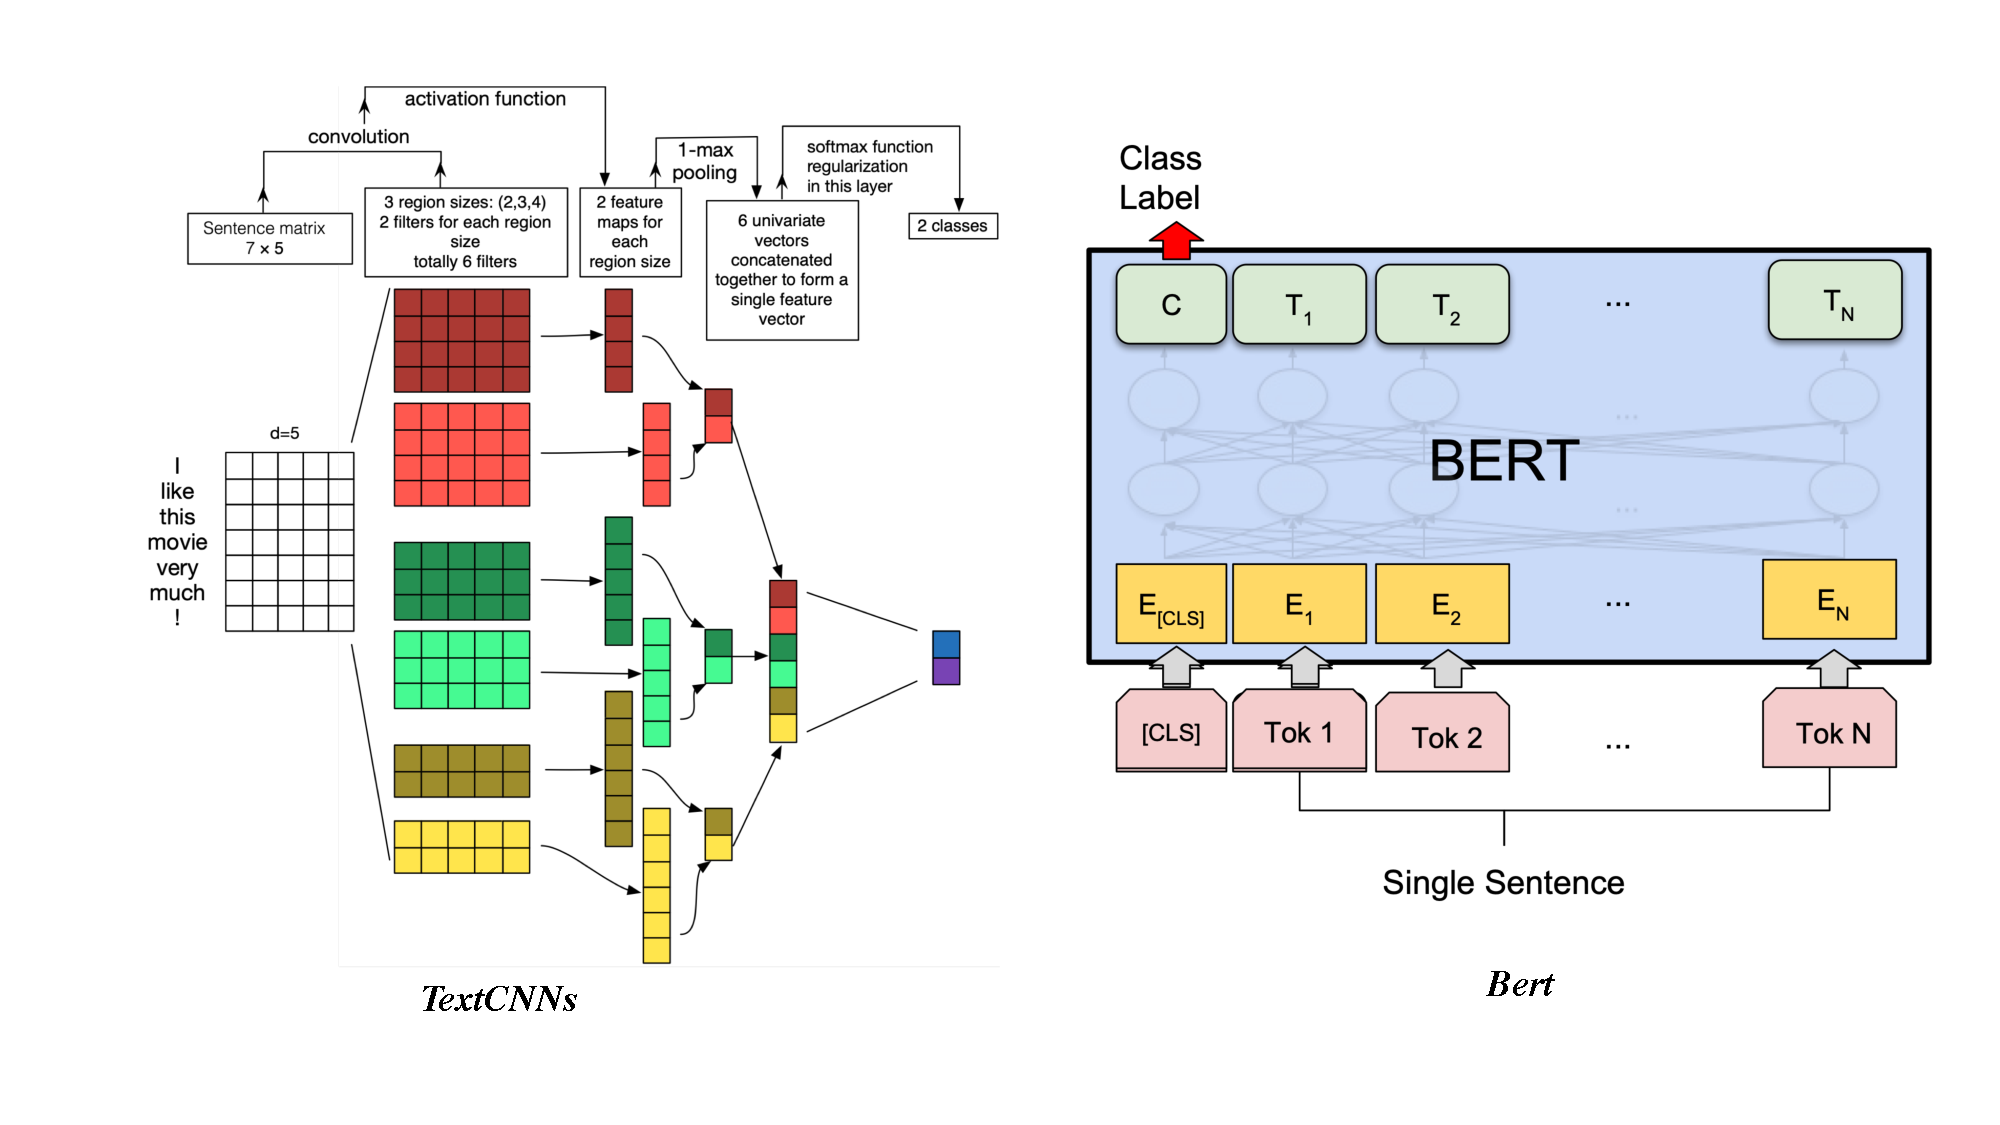
\includegraphics[width=\textwidth]{figures/figure.pdf}
%     \end{center}
%     \caption{Two model in this paper, TextCNN \& Bert}
%     \label{fig:model}
% \end{figure*}


\subsection{Bi-LSTM}
\label{sec:lstm}

Recurrent neural networks (RNNs) are a family of neural networks that operate on sequential data. They take as input a sequence of vectors $(\mathbf{x}_1, \mathbf{x}_2, \ldots, \mathbf{x}_n)$ and return another sequence $(\mathbf{h}_1, \mathbf{h}_2, \ldots, \mathbf{h}_n)$ that represents some information about the sequence at every step in the input. Although RNNs can, in theory, learn long dependencies, in practice they fail to do so and tend to be biased towards their most recent inputs in the sequence. Long Short-term Memory Networks (LSTMs) have been designed to combat this issue by incorporating a memory-cell and have been shown to capture long-range dependencies. They do so using several gates that control the proportion of the input to give to the memory cell, and the proportion from the previous state to forget.
We use the following implementation:
\\
\begin{align*}
\mathbf{i}_{t} &= \sigma(\mathbf{W}_{xi}\mathbf{x}_{t} + \mathbf{W}_{hi}\mathbf{h}_{t-1} + \mathbf{W}_{ci}\mathbf{c}_{t-1} + \mathbf{b}_{i})\\
% \mathbf{f}_{t} &= \sigma(\mathbf{W}_{xf}\mathbf{x}_{t} + \mathbf{W}_{hf}\mathbf{h}_{t-1}+\mathbf{W}_{cf}\mathbf{c}_{t-1} + \mathbf{b}_{f})\\
\mathbf{c}_{t} &= (1 - \mathbf{i}_{t})\odot\mathbf{c}_{t-1} +\\
&\qquad \mathbf{i}_{t}\odot \tanh(\mathbf{W}_{xc}\mathbf{x}_{t} + \mathbf{W}_{hc}\mathbf{h}_{t-1} + \mathbf{b}_{c})\\
\mathbf{o}_{t} &= \sigma(\mathbf{W}_{xo}\mathbf{x}_{t} + \mathbf{W}_{ho}\mathbf{h}_{t-1} + \mathbf{W}_{co}\mathbf{c}_{t} + \mathbf{b}_{o})\\
\mathbf{h}_{t} &= \mathbf{o}_{t}\odot\tanh(\mathbf{c}_{t}),
\end{align*}
where $\sigma$ is the element-wise sigmoid function, and $\odot$ is the element-wise product.

For a given sentence $(\mathbf{x}_1, \mathbf{x}_2, \ldots, \mathbf{x}_n)$ containing $n$ words, each represented as a $d$-dimensional vector, an LSTM computes a representation $\overrightarrow{\mathbf{h}_t}$ of the left context of the sentence at every word $t$. Naturally, generating a representation of the right context $\overleftarrow{\mathbf{h}_t}$ as well should add useful information. This can be achieved using a second LSTM that reads the same sequence in reverse. We will refer to the former as the forward LSTM and the latter as the backward LSTM. These are two distinct networks with different parameters. This forward and backward LSTM pair is referred to as a bidirectional LSTM.

The representation of a word using this model is obtained by concatenating its left and right context representations, $\mathbf{h}_{t} = [\overrightarrow{\mathbf{h}_{t}} ; \overleftarrow{\mathbf{h}_{t}}]$. These representations effectively include a representation of a word in context, which is useful for numerous tagging applications.

\subsection{CRF Tagging Models}
\label{sec:crf}

A very simple---but surprisingly effective---tagging model is to use the $\mathbf{h}_t$'s as features to make independent tagging decisions for each output $y_t$. Despite this model's success in simple problems like POS tagging, its independent classification decisions are limiting when there are strong dependencies across output labels. NER is one such task, since the ``grammar'' that characterizes interpretable sequences of tags imposes several hard constraints (e.g., I-PER cannot follow B-LOC; see \S\ref{IOBES} for details) that would be impossible to model with independence assumptions.

Therefore, instead of modeling tagging decisions independently, we model them jointly using a conditional random field. For an input sentence
$$\mathbf{X} = (\mathbf{x}_1, \mathbf{x}_2, \ldots, \mathbf{x}_n),$$
we consider $\mathbf{P}$ to be the matrix of scores output by the bidirectional LSTM network. $\mathbf{P}$ is of size $n~\times~k$, where $k$ is the number of distinct tags, and $P_{i, j}$ corresponds to the score of the $j^{th}$ tag of the $i^{th}$ word in a sentence. For a sequence of predictions
$$\mathbf{y} = (y_1, y_2, \ldots, y_n),$$
we define its score to be
$$s(\mathbf{X}, \mathbf{y})=\sum_{i=0}^{n} A_{y_i, y_{i+1}} + \sum_{i=1}^{n} P_{i, y_i}$$
where $\mathbf{A}$ is a matrix of transition scores such that $A_{i, j}$ represents the score of a transition from the tag $i$ to tag $j$. $y_0$ and $y_n$ are the \textit{start} and \textit{end} tags of a sentence, that we add to the set of possible tags. $\mathbf{A}$ is therefore a square matrix of size $k+2$.
\\
\\
A softmax over all possible tag sequences yields a probability for the sequence $\mathbf{y}$:
$$p(\mathbf{y} | \mathbf{X}) = \frac{
	e^{s(\mathbf{X}, \mathbf{y})}
}{
	\sum_{\mathbf{\widetilde{y}} \in \mathbf{Y_X}} e^{s(\mathbf{X}, \mathbf{\widetilde{y}})}
}.$$
During training, we maximize the log-probability of the correct tag sequence:

\subsection{Bert}


\begin{figure*}[t]
    \begin{center}
        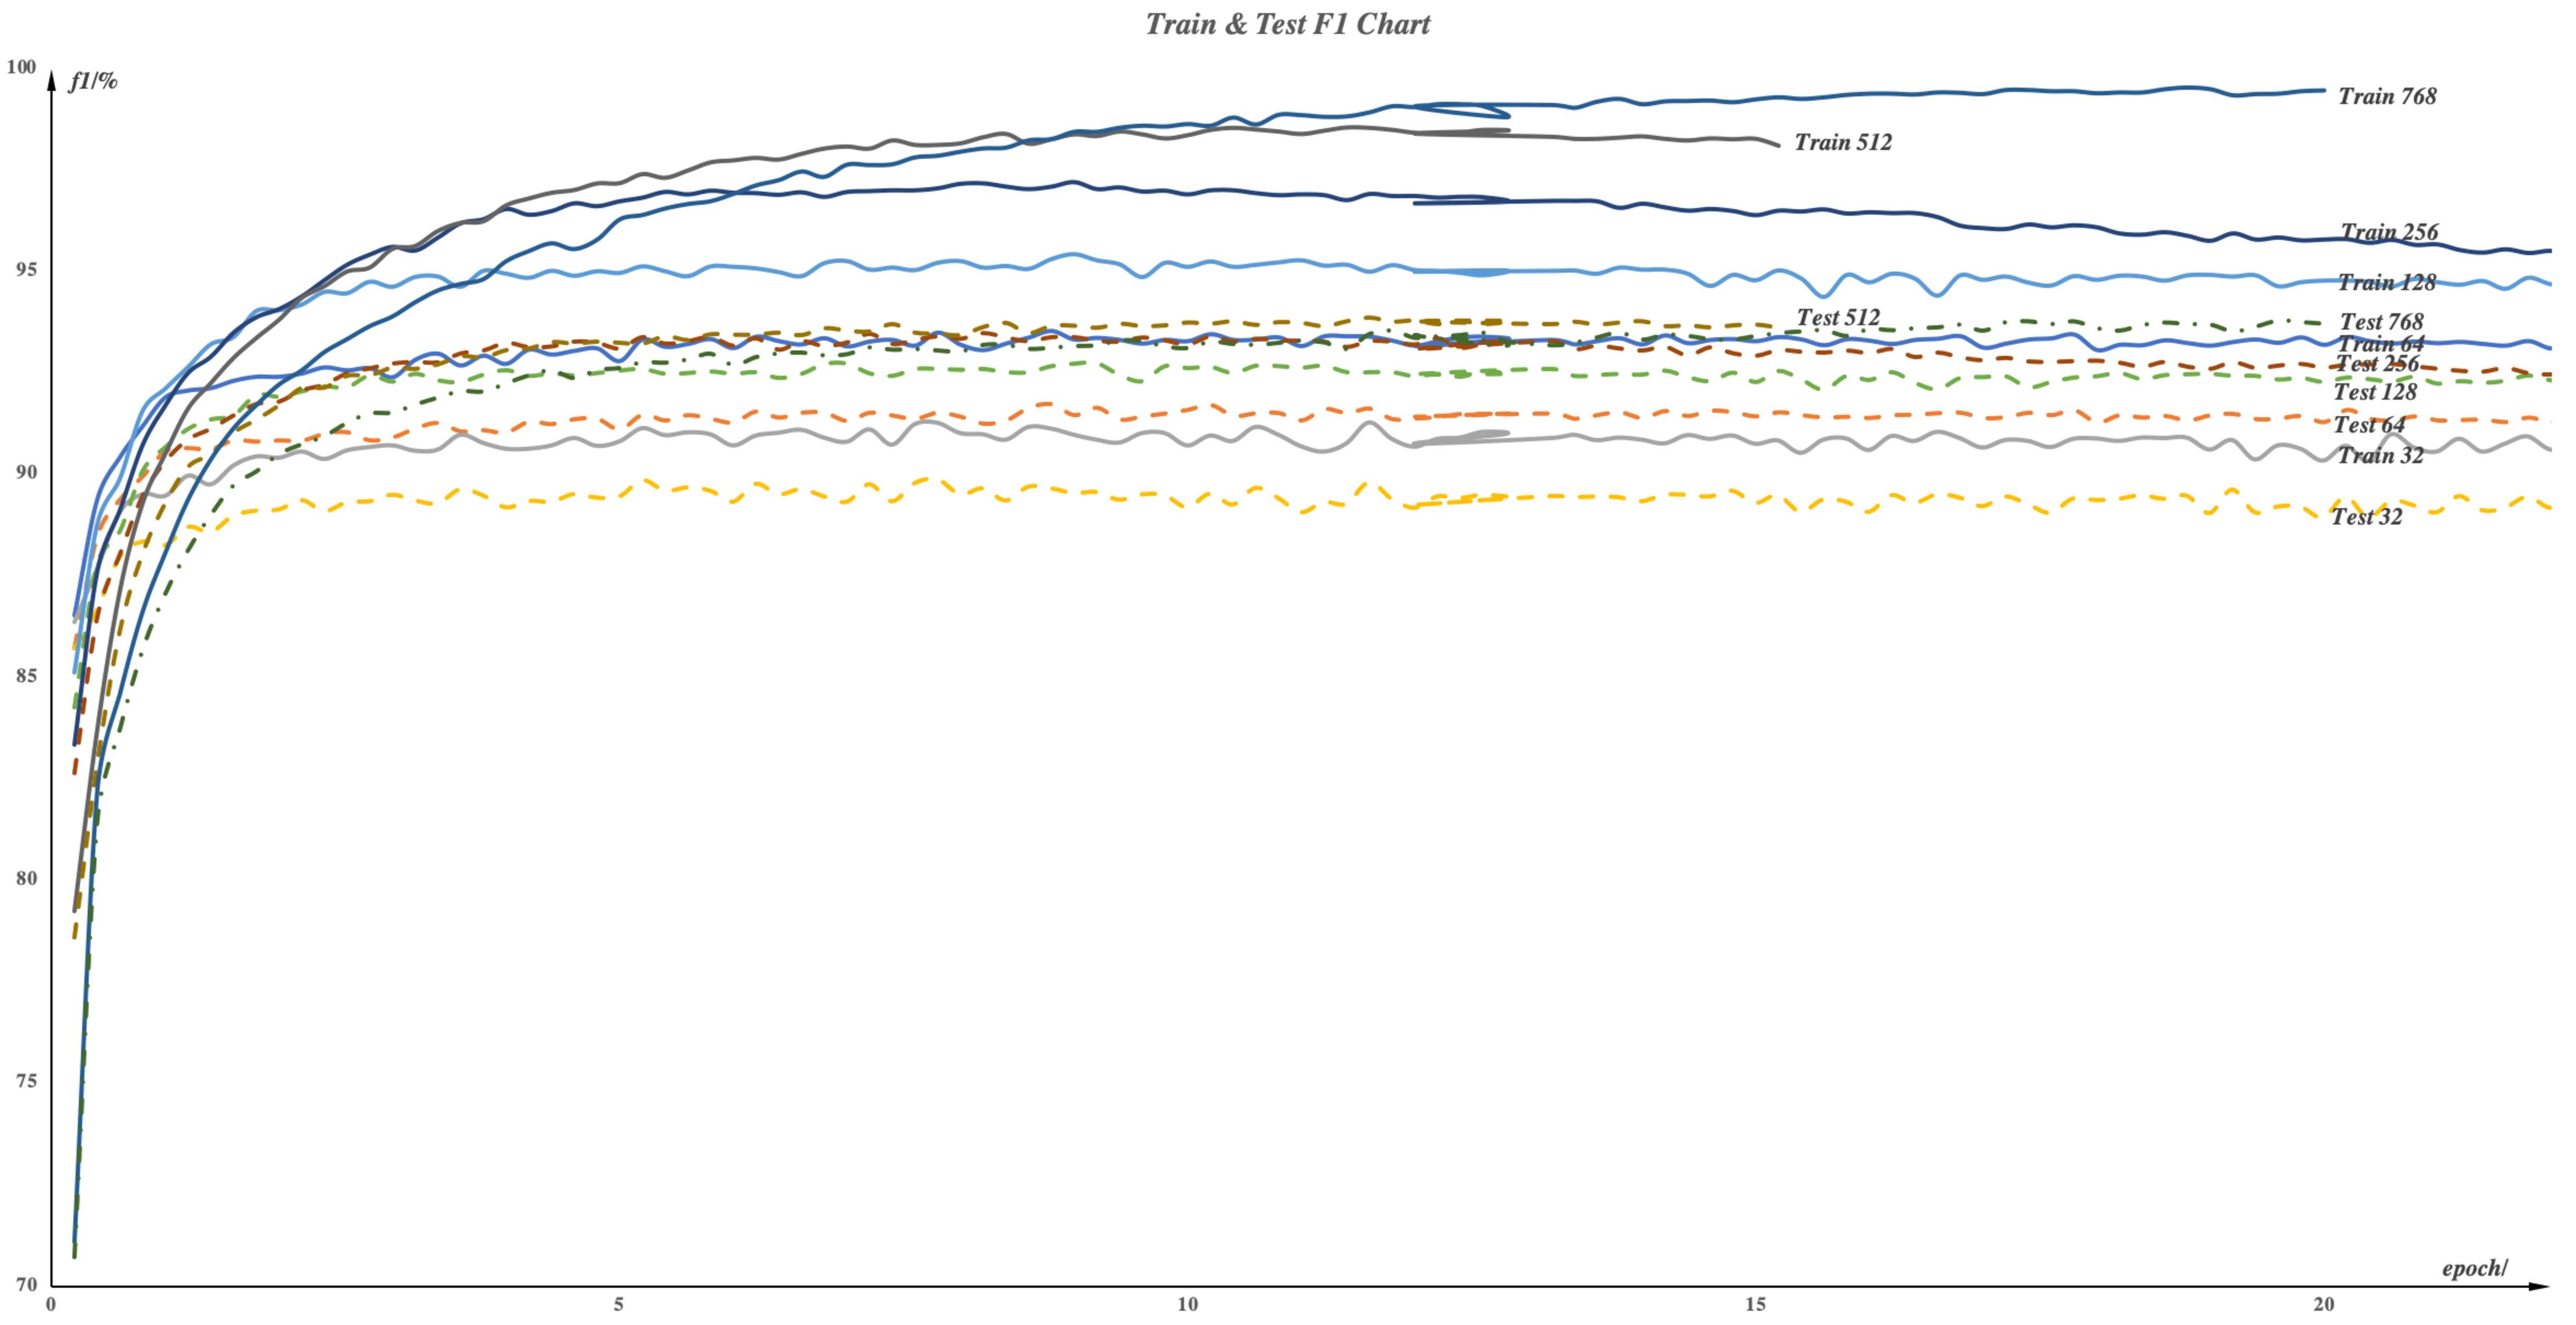
\includegraphics[width=\textwidth]{figures/batch.pdf}
    \end{center}
    \caption{Train Set & Dev Set epoch \& F1 distribute in CWS problem}
    \label{fig:model}
\end{figure*}
\end{figure*}
\begin{figure*}[t]
    \begin{center}
        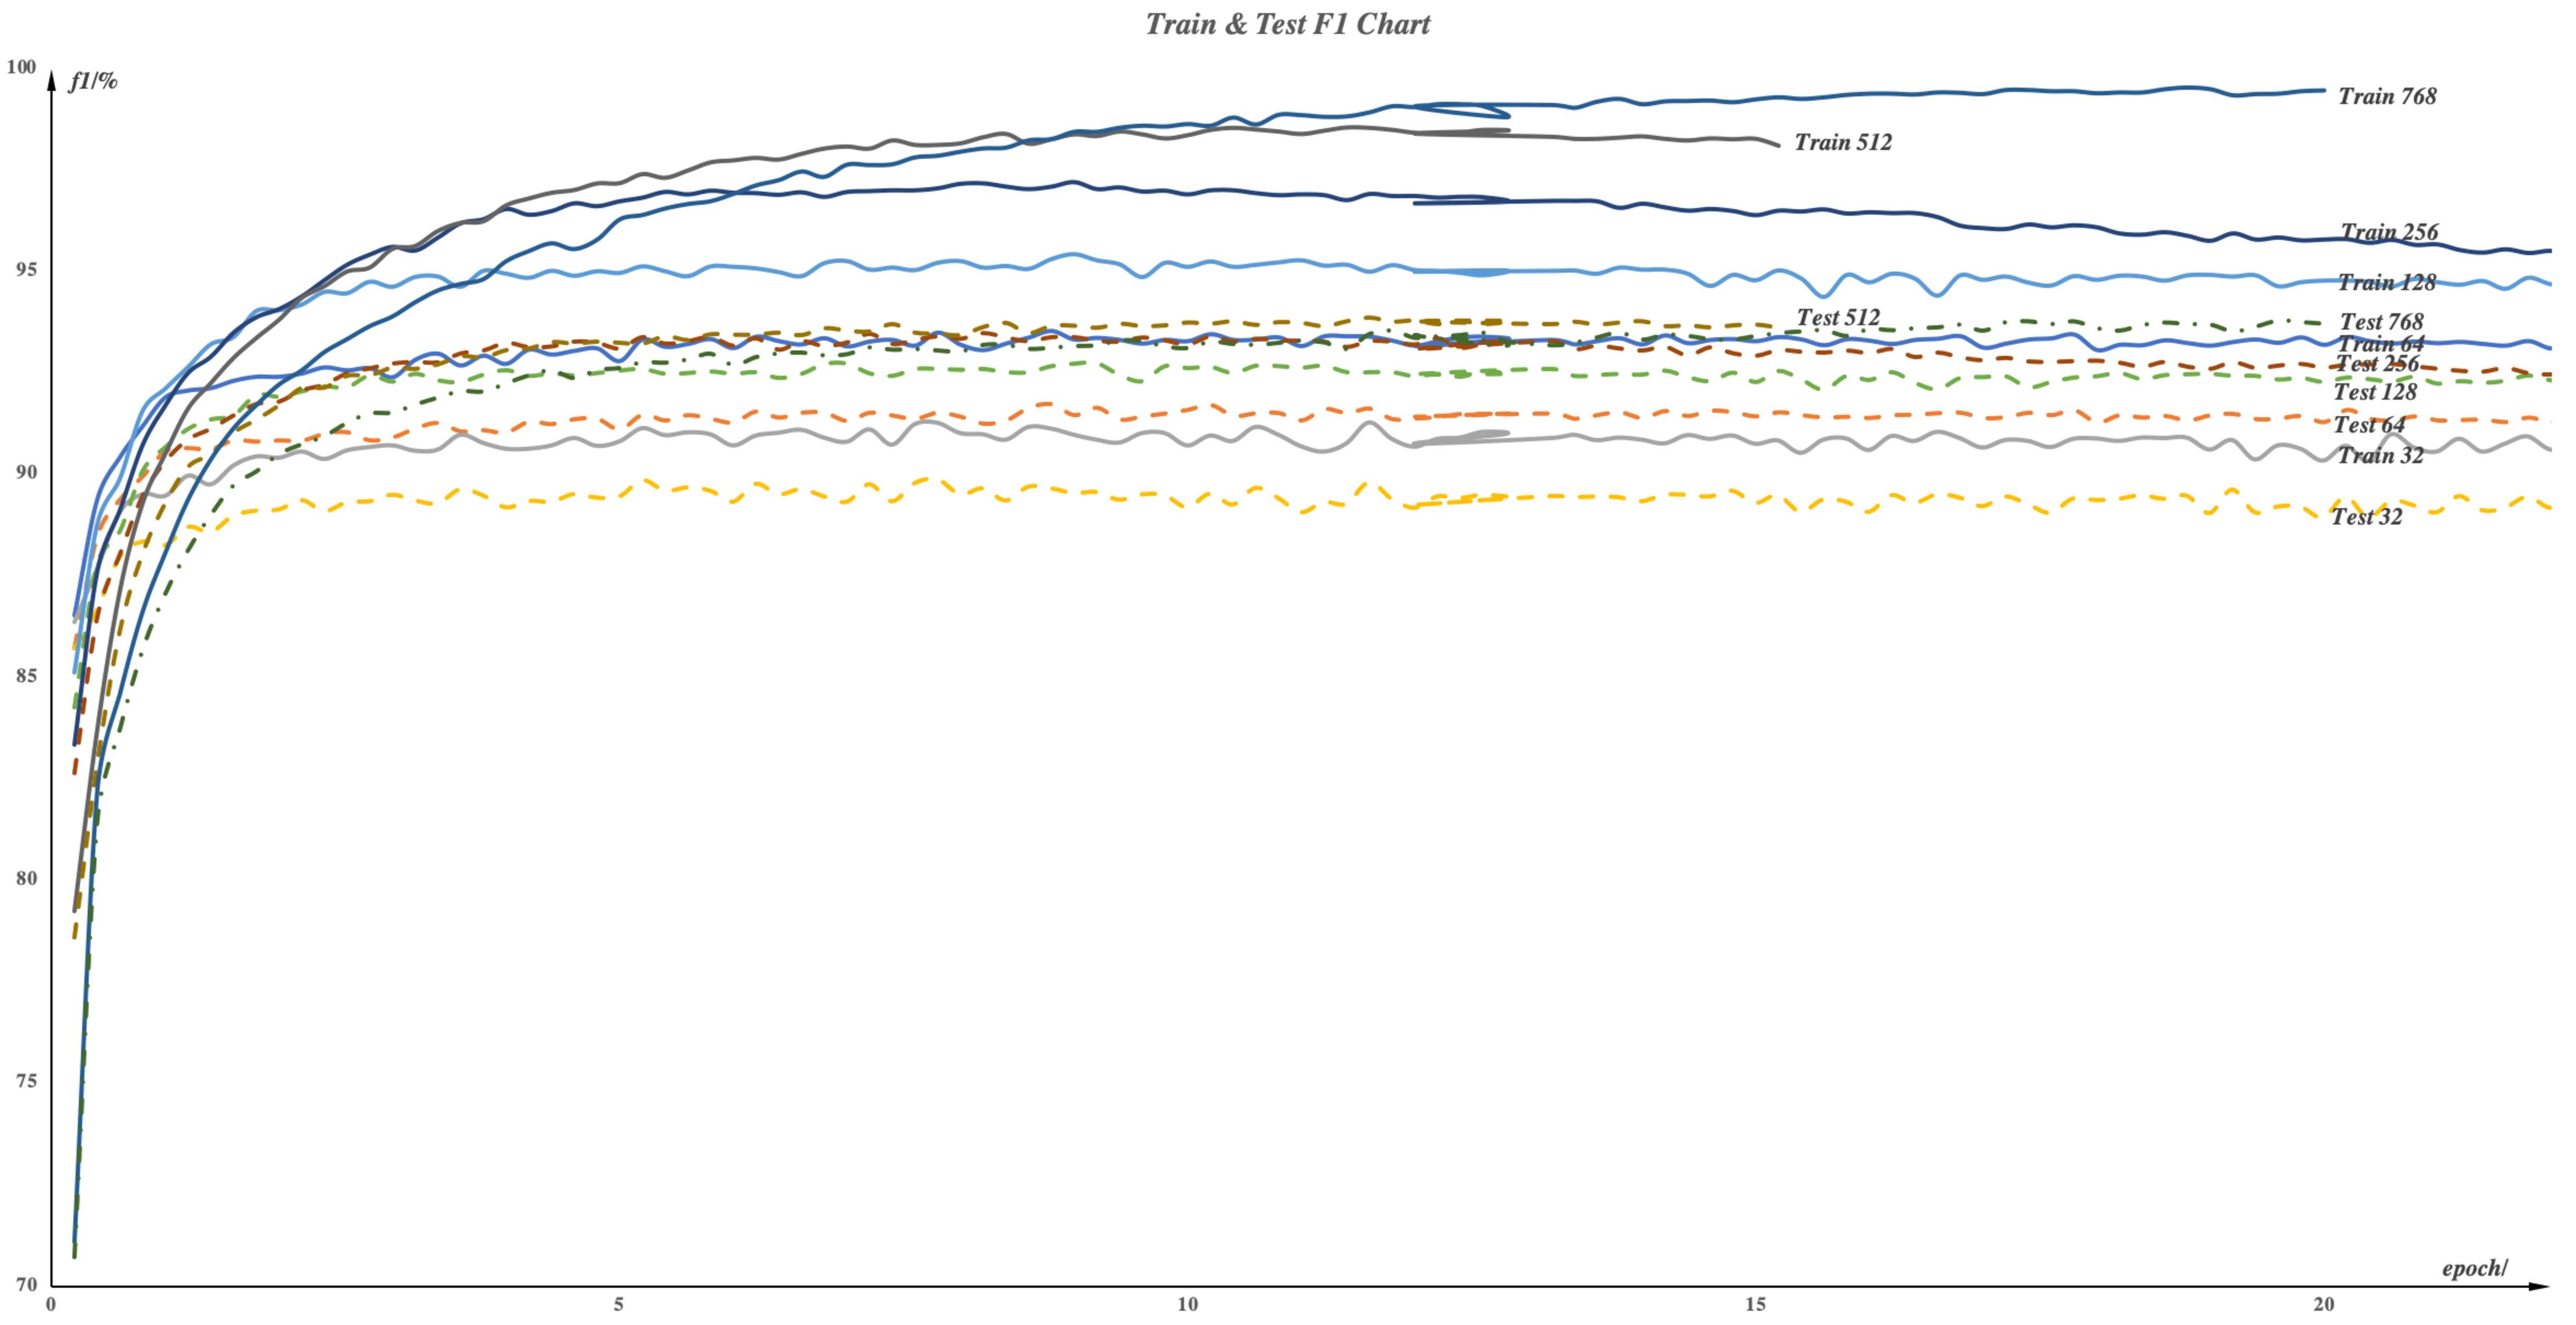
\includegraphics[width=\textwidth]{figures/batch.pdf}
    \end{center}
    \caption{Train Set & Dev Set epoch \& F1 distribute in NER problem}
    \label{fig:model}
\end{figure*}
\end{figure*}
\begin{table*}[htbp!]
    \centering
    \begin{tabular}{lccccc}
    \midrule
    Type  &  Train Set Num          & Train Set Percent \%         & Dev Set Num       & Dev Set Percent \%\\
    \midrule
    N     & 1125991       & 90.63               & 479394      & 90.46             \\
    B-LOC & 25211         & 2.03                & 11002       & 2.08              \\
    I-LOC & 32022         & 2.58                & 13973       & 2.64              \\
    B-ORG & 9428          & 0.76                & 4062        & 0.77              \\
    I-ORG & 15220         & 1.23                & 6605        & 1.23              \\
    B-PER & 11562         & 0.93                & 4990        & 0.94              \\
    I-PER & 22858         & 1.84                & 9884        & 1.87              \\

    \bottomrule
    \end{tabular}
\caption{Chinese Traditional Corps Distributed(in \%)}
\label{tab:text_cnn}
\end{table*}

\begin{table*}[htbp!]
    \centering
    \begin{tabular}{lccccccc}
    \midrule
    Batch Size  &  Train P          & Train R        & Train F1       & Dev P      & Dev R & Dev F1 & Best Epoch\\
    \midrule
    \underline{\bf64}& 99.75   & 99.76   & 99.76    & 86.95 & 81.30 & \bf84.03  & 30         \\
    256        & 97.75   & 96.59   & 97.17    & 84.56 & 79.27 & 81.83     & 33         \\
    512        & 94.75   & 92.12   & 93.42    & 83.54 & 78.14 & 80.75     & 36         \\
    768        & 88.41   & 83.74   & 86.02    & 81.36 & 75.80 & 78.48     & 38         \\

    \bottomrule
    \end{tabular}
\caption{Comparison between different Batch Size of BiLSTM CRF Model in NER Problem on Chinese traditional Corps data (in \%)}
\label{tab:batchSize2}
\end{table*}

\begin{table*}[htbp!]
    \centering
    \begin{tabular}{lccccc}
    \midrule
    Type  &  Train Set Num          & Train Set Percent \%         & Dev Set Num       & Dev Set Percent \%\\
    \midrule
    N     & 1125991       & 90.63               & 479394      & 90.46             \\
    B-LOC & 25211         & 2.03                & 11002       & 2.08              \\
    I-LOC & 32022         & 2.58                & 13973       & 2.64              \\
    B-ORG & 9428          & 0.76                & 4062        & 0.77              \\
    I-ORG & 15220         & 1.23                & 6605        & 1.23              \\
    B-PER & 11562         & 0.93                & 4990        & 0.94              \\
    I-PER & 22858         & 1.84                & 9884        & 1.87              \\

    \bottomrule
    \end{tabular}
\caption{Chinese Traditional Corps Distributed(in \%)}
\label{tab:text_cnn}
\end{table*}

\begin{table*}[htbp!]
    \centering
    \begin{tabular}{lccccccccc}
    \midrule
    problem & Hidden Size  &  Embed Size  & Train P   & Train R     & Train F1    & Dev P      & Dev R & Dev F1 & Best Epoch\\
    \midrule
   
    CWS & 512         & 256        & 93.53   & 93.54   & 93.53    & 91.65 & 91.78 & 91.71     & 8.8        \\
    CWS & 512         & 512        & 91.81   & 91.92   & 91.86    & 90.38 & 90.56 & 90.47     & 3.8        \\
    CWS & \underline{\bf768}& \underline{\bf256}        & 93.51   & 93.94   & 93.72    & 91.50 & 92.03 & \bf91.77  & 10.8       \\
    NER & 512         & 256        & 99.75   & 99.76   & 99.76    & 86.95 & 81.30 & 84.03     & 30         \\
    NER & \underline{\bf300}& \underline{\bf300}& 99.00   & 97.76   & 98.38    & 87.38 & 81.10 & \bf84.13  & 25         \\

    \bottomrule
    \end{tabular}
\caption{Comparison between different Hyper-params of BiLSTM CRF Model in CWS \& NER Problem on Chinese traditional Corps data (in \%)}
\label{tab:batchSize}
\end{table*}

\begin{table*}[htbp!]
    \centering
    \begin{tabular}{lccccccc}
    \midrule
    Epoch & Dev Acc & Dev P & Dev R & Dev F1    & Loc F1 & Org F1 & Per F1\\
    \midrule
    1     & 99.63   & 95.28 & 96.42 & 95.85     & 97.68  & 91.88  & 98.05  \\
    2     & 99.67   & 96.30 & 96.97 & 96.64     & 98.02  & 94.04  & 98.20  \\
    \underline{\bf3}& \bf99.70 & 96.62 & 97.23  & \bf96.92  & 98.31& 94.48  & 98.55  \\
    \bottomrule
    \end{tabular}
\caption{Bert Result in My Test Work (in \%)}
\label{tab:batchSize}
\end{table*}

\begin{table*}[htbp!]
    \centering
    \begin{tabular}{lcccccccc}
    \midrule
    problem & Model & Train P   &Train R     & Train F1       & Dev P      & Dev R & Dev F1 &Best Epoch\\
    \midrule
    CWS& BiLSTM + CRF & 98.36   & 98.42   & 98.39    & 93.70 & 93.82 &  93.76 & 12           \\
    CWS& \underline{\bf Bert + CRF}   & -       & -       & -        & 97.97 & 97.60 &  \bf97.78 & 1(only test) \\
    NER& BiLSTM + CRF & 99.75   & 99.76   & 99.76    & 86.95 & 81.30 & 84.03 & 30         \\
    NER& \underline{\bf Bert + CRF}   & -       & -       & -        & 96.62 & 97.23 & \bf96.92 & 3         \\     

    \bottomrule
    \end{tabular}
\caption{Best Result in My Test Work (in \%)}
\label{tab:batchSize}
\end{table*}



BERT is one of the key innovations in the recent progress of contextualized representation learning \cite{peters2018deep,howard2018universal,radford2018improving,devlin2018bert}.
The idea behind the progress is that even though the word embedding layer (in a typical neural network for NLP) is trained from large-scale corpora, training a wide variety of neural architectures that encode contextual representations only from the limited supervised data on end tasks is insufficient.
Unlike ELMo \cite{peters2018deep} and ULMFiT \cite{howard2018universal} that are intended to provide additional features for a particular architecture that bears human's understanding of the end task, BERT adopts a fine-tuning approach that requires almost no specific architecture for each end task. This is desired as an intelligent agent should minimize the use of prior human knowledge in the model design. Instead, it should learn such knowledge from data. BERT has two parameter intensive settings: 


\begin{itemize}
    \item {\bf \bertbase}: L=12, H=768, A=12, Total Parameters=110M
    \item {\bf \bertlarge}: L=24, H=1024, A=16, Total Parameters=340M
\end{itemize}

\section{Experiments}
\label{sec:experiments}

In this section, we experiment for two model(BiLSTM + CRF/Bert + CRF).\ref{fig:model} for two sequence annotation problem in a chinese traditional corps.

And I also analysis the corps distribution, It means we can't use single classify model to deal this problem.

\subsection{BiLSTM CRF Batch Size}
\label{sec:BiLSTM CRF Batch Size}

In this experiment, I set the hidden dim size as 512, embed size as 256, the learning rate of cws is 0.01, the learning rate of NER is 0.001.
And when the batch size has been increased, the f1 score in dev Set have been increased too in CWS problem. \ref{fig:batch}
But I find the rule have been reverse in NER problem.\ref{fig:batch2} It may cause by the diff of learning rate. I thought the also show that cws is only a surface layer extract problem.

\subsection{Some Hyper-Params}
\label{sec:hyper params} 

Except experiment batch size, I also test for hidden state size, Embed Size.
And I find In CWS problem, The bigger Hidden State size may import train effect.
And this also mean that the epoch to best is become large.

\subsection{Bert}
\label{sec:bert}

Compare with pre-training Bert with fine-tune Bert, the score significantly Improve.
The position embedding \& Transformer construction work well to obtain information in context.
Bert result is very outstanding, In CWS problem, Bert Improve 4\% in dev set of f1. In Ner problem, Bert Improve 13\% point in Dev Set of offset.
 



\section{Conclusion}
\label{sec:Conclusion}
In this paper, we introduce two deep-learning sequence annotation model. Both BiLstm + CRF and Bert-CRF well in this task. And Bert can get more semantic info on context.
The pad position also has some effect on this model.
I achieve a 97.60\% Recall score on CWS,  Macro-F1 is 97.78\% by using Bert CRF, And in NER,  I achieve a 93.32\% Recall score on NER,  Macro-F1 is 96,92\% by using Bert CRF.
Every score is better than the rank 1 in the competition. 

\bibliographystyle{acl_natbib}
\bibliography{mybib}

\end{document}
